\documentclass[12pt]{article}
\usepackage[a4paper, margin=0.75in]{geometry}
\usepackage[document]{ragged2e}
\usepackage{graphicx}
\usepackage{subfig}
\graphicspath{ {./images/} }
\usepackage{enumerate}
\usepackage{framed}
\usepackage{amsmath,amsfonts,amsthm,thmtools,amssymb,mathtools,commath}
\usepackage{physics}
\usepackage{tikz}
\usetikzlibrary{mindmap}
\usepackage{caption}
\usepackage{xcolor}
\usepackage[most]{tcolorbox}
\usepackage{cleveref}


%%%%%%%%%%%%%%%%
%  Definition  %
%%%%%%%%%%%%%%%%
\tcbuselibrary{theorems,skins,hooks}
\newtcbtheorem[number within=subsection]{definition}{Definition}%
{
    % theorem style=definition,
    enhanced,
	before skip=2mm,after skip=2mm, colback=cyan!5,colframe=cyan!80!black,boxrule=0.5mm,
	attach boxed title to top left={xshift=1cm,yshift*=1mm-\tcboxedtitleheight},
	boxed title style={frame code={
					\path[fill=cyan]
					([yshift=-1mm,xshift=-1mm]frame.north west)
					arc[start angle=0,end angle=180,radius=1mm]
					([yshift=-1mm,xshift=1mm]frame.north east)
					arc[start angle=180,end angle=0,radius=1mm];
					\path[left color=cyan!30!black,right color=cyan!30!black,
						middle color=cyan!50!black]
					([xshift=-2mm]frame.north west) -- ([xshift=2mm]frame.north east)
					[rounded corners=1mm]-- ([xshift=1mm,yshift=-1mm]frame.north east)
					-- (frame.south east) -- (frame.south west)
					-- ([xshift=-1mm,yshift=-1mm]frame.north west)
					[sharp corners]-- cycle;
				},interior engine=empty,
		},
	fonttitle=\bfseries,
	title={#2},#1
}{def}


%%%%%%%%%%%%%
%  Theorem  %
%%%%%%%%%%%%%
\tcbuselibrary{theorems,skins,hooks}
\newtcbtheorem[use counter from=definition]{theorem}{Theorem}%
{
    theorem style=plain,
    enhanced,
    colframe=green,
    boxrule=1pt,
    titlerule=0mm,
    toptitle=1mm,
    bottomtitle=1mm,
    fonttitle=\bfseries,
    fontupper=\mdseries\itshape,
    coltitle=green!30!black,
    colbacktitle=cyan!15!white,
    colback=green!10,
    description font=\bfseries\sffamily
}{thrm}


%%%%%%%%%%%%%%
% Corollary  %
%%%%%%%%%%%%%%
 \tcbuselibrary{theorems,skins}
 \newtcbtheorem[use counter from=theorem]{corollary}{Corollary}%
 {
    theorem style=plain,
    enhanced,
    colframe=green,
    frame hidden,
    titlerule=0mm,
    toptitle=1mm,
    bottomtitle=1mm,
    fonttitle=\bfseries,
    fontupper=\mdseries\itshape,
    coltitle=green!30!black,
    colbacktitle=cyan!15!white,
    colback=green!10,
    description font=\bfseries\sffamily
 }{corl}


%%%%%%%%%%%%%
%  Example  %
%%%%%%%%%%%%%
\tcbuselibrary{theorems,skins,hooks}
\newtcbtheorem[number within=section]{example}{Example}%
{
	enhanced,
	breakable,
	colback = gray!5,
	frame hidden,
	boxrule = 0sp,
	borderline west = {2pt}{0pt}{gray},
	sharp corners,
	detach title,
	before upper = \tcbtitle\par\smallskip,
    coltitle=gray!70!black,
	fonttitle = \bfseries\sffamily,
	description font = \mdseries\bfseries
}
{xmp}


%%%%%%%%%%%%%%
%  Exercise  %
%%%%%%%%%%%%%%
\tcbuselibrary{theorems,skins,hooks}
\newtcbtheorem[number within=section]{exercise}{Exercise}%
{
    enhanced,
    breakable,
    colback=black!5,
    colframe=black!30,
    left=0.5em,
    before skip=10pt,
    after skip=10pt,
    boxrule=0pt,
    boxsep=0pt,
    arc=0pt,
    outer arc=0pt,
    borderline west={3pt}{0pt}{black!30},
}{exc}

%%%%%%%%%%
%  Note  %
%%%%%%%%%%
\usetikzlibrary{arrows,calc,shadows.blur}
\tcbuselibrary{skins}
\newtcolorbox{note}[1][]{%
	enhanced jigsaw,
	colback=gray!20!white,%
	colframe=gray!80!black,
	size=small,
	boxrule=1pt,
	title=\textbf{Note:-},
	halign title=flush center,
	coltitle=black,
	breakable,
	drop shadow=black!50!white,
	attach boxed title to top left={xshift=1cm,yshift=-\tcboxedtitleheight/2,yshifttext=-\tcboxedtitleheight/2},
	minipage boxed title=1.5cm,
	boxed title style={%
			colback=white,
			size=fbox,
			boxrule=1pt,
			boxsep=2pt,
			underlay={%
					\coordinate (dotA) at ($(interior.west) + (-0.5pt,0)$);
					\coordinate (dotB) at ($(interior.east) + (0.5pt,0)$);
					\begin{scope}
						\clip (interior.north west) rectangle ([xshift=3ex]interior.east);
						\filldraw [white, blur shadow={shadow opacity=60, shadow yshift=-.75ex}, rounded corners=2pt] (interior.north west) rectangle (interior.south east);
					\end{scope}
					\begin{scope}[gray!80!black]
						\fill (dotA) circle (2pt);
						\fill (dotB) circle (2pt);
					\end{scope}
				},
		},
	#1,
}

\usepackage[scr]{rsfso}
\usepackage{physics}
\usepackage{multicol}
\renewcommand{\arraystretch}{2.5}

\newcommand{\Lap}{\mathscr{L}}
\newcommand{\Lapinv}{\mathscr{L}^{-1}}

\numberwithin{equation}{subsection}

\title{
    \textbf{Fourier Analysis}
}

\author{
    Turja Roy\\
    ID: 2108052
}
\date{}

\begin{document}
\maketitle
\tableofcontents
\newpage

%%%%%%%%%%%%%%%%%%
%  Introduction  %
%%%%%%%%%%%%%%%%%%

\section{Introduction}

\subsection{Periodic Functions}
\begin{definition}{Periodic Functions}{}
    A function $f(x)$ is said to be have a \textit{period} $P$ or to be \textit{periodic} with period $P$ if for all $x$, $f(x+P) = f(x)$ where $P$ is a positive constant. The least value of $P>0$ is called the \textit{least period} or simply the \textit{period} of $f(x)$.
\end{definition}
\begin{example}{Some examples of periodic functions}{}
    \begin{enumerate}
        \item $\sin{x}$ has periods $2\pi, 4\pi, 6\pi, \cdots$ and $-\pi, -3\pi, -5\pi, \cdots$ and hence the least period is $2\pi$.\\
        \item $\cos{x}$ has the least period $2\pi$.\\
        \item $\tan{x}$ has the least period $\pi$.
    \end{enumerate}
    Some other examples:\\
    \begin{minipage}{.3\textwidth}
        \renewcommand{\thefigure}{1.1.1}
        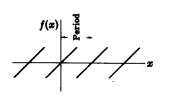
\includegraphics[scale=0.8]{./images/1.1.1.png}
        \captionof{figure}{}
    \end{minipage}
    \begin{minipage}{.3\textwidth}
        \renewcommand{\thefigure}{1.1.2}
        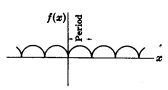
\includegraphics[scale=0.8]{./images/1.1.2.png}
        \captionof{figure}{}
    \end{minipage}
    \begin{minipage}{.35\textwidth}
        \renewcommand{\thefigure}{1.1.3}
        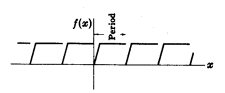
\includegraphics[scale=0.74]{./images/1.1.3.png}
        \captionof{figure}{}
    \end{minipage}
\end{example}

\subsection{Piecewise Continuous Functions}
\begin{definition}{Piecewise Continuous Functions}{}
    A function $f(x)$ is said to be \textit{piecewise continuous} in the interval $[a,b]$ if $f(x)$ is continuous in the interval $(a,b)$ and has a finite number of finite discontinuities in the interval $[a,b]$.
\end{definition}

\renewcommand{\thefigure}{1.2.1}
\begin{figure}[htpb]
    \centering
    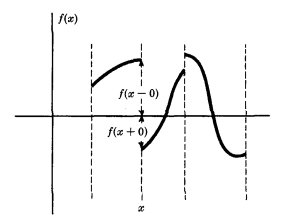
\includegraphics[width=0.4\textwidth]{./images/1.2.1}
    \caption{}
    \label{fig:1.2.1}
\end{figure}

The right-hand limit of $f(x)$ is often denoted by $\lim_{\epsilon \to 0} f(x+\epsilon) = f(x+0)$, where $\epsilon > 0$.\\
Similarly, the left-hand limit of $f(x)$ is denoted by $\lim_{\epsilon \to 0} f(x-\epsilon) = f(x-0)$, where $\epsilon > 0$. The values of $f(x+0)$ and $f(x-0)$ at the point $x$ in (\ref{fig:1.2.1}) are as indicated.


%%%%%%%%%%%%%%%%%%%%%%%
%  Fourier Expansion  %
%%%%%%%%%%%%%%%%%%%%%%%
\section{Fourier Expansion}

\subsection{Definition}
\begin{definition}{Fourier Expansion}{}
    Let $f(x)$ be defined in the interval $(-L,L)$ and determined outside of this interval by $f(x+2L)=f(x)$, i.e. assume that $f(x)$ has the period $2L$. The \textit{Fourier series} or \textit{Fourier expansion} corresponding to $f(x)$ is defined to be
    \begin{equation}
        f(x) = \frac{a_0}{2} + \sum_{n=1}^{\infty} \left[ a_n \cos \left( \frac{n\pi x}{L} \right) + b_n \sin \left( \frac{n\pi x}{L} \right) \right]
    \end{equation}
    where the \textit{Fourier coefficients} $a_n$ and $b_n$ are given by
    \begin{equation}
        \begin{cases}
            \displaystyle 
            a_0 = \frac{1}{L} \int_{-L}^{L} f(x) dx \\\\
            \displaystyle 
            a_n = \frac{1}{L} \int_{-L}^{L} f(x) \cos \left( \frac{n\pi x}{L} \right) dx \qquad n = 0, 1, 2, \cdots \\\\
            \displaystyle 
            b_n = \frac{1}{L} \int_{-L}^{L} f(x) \sin \left( \frac{n\pi x}{L} \right) dx
        \end{cases}
    \end{equation}
\end{definition}

\subsection{Some pre-derivations}

\begin{align*}
    I &= \int_{-L}^{L} {\sin^2{\frac{n\pi x}{L}}} \: d{x} \\
    &= \sin{\frac{n\pi x}{L}} \cdot \frac{L}{n\pi} (\cos{n\pi} - \cos{n\pi}) + \frac{n\pi}{L}\cdot\frac{L}{n\pi} \int_{-L}^{L} {\cos{\frac{n\pi x}{L}}\cos{\frac{n\pi x}{L}}} \: d{x} \\
    &= \int_{-L}^{L} {\cos^2{\frac{n\pi x}{L}}} \: d{x} \\
    &= \frac{1}{2} \int_{-L}^{L} {\left( \cos{\frac{2n\pi x}{L} + 1} \right)} \: d{x} \\
    &= \frac{1}{2} \int_{-L}^{L} {\cos{\frac{2n\pi x}{L}}} \: d{x} + \frac{1}{2} \int_{-L}^{L} {} \: d{x} \\
    &= 0 + \frac{1}{2} \cdot 2L \\
    &= L \\
\end{align*}
\begin{align*}
    I_1 &= \int_{-L}^{L} {\cos{\frac{m\pi x}{L}} \cos{\frac{n\pi x}{L}}} \: d{x} \qquad [m \neq 0] \\
    &= \cos{\frac{m\pi x}{L}} \int_{-L}^{L} {\cos{\frac{n\pi x}{L}}} \: d{x} + \frac{m}{n} \int_{-L}^{L} {\sin{\frac{m\pi x}{L}} \sin{\frac{n\pi x}{L}}} \: d{x} \\
    &= \frac{L}{n\pi} \cos{\frac{m\pi x}{L}} (\sin{n\pi} + \sin{n\pi}) + \frac{m}{n} I_2 \\
    &= 0 + \frac{m}{n} \left[ \int_{-L}^{L} {\sin{\frac{m\pi x}{L}} \sin{\frac{n\pi x}{L}}} \: d{x} \right] \\
    &= \frac{m}{n} \left[ \sin{\frac{m\pi x}{L}} \int_{-L}^{L} {\sin{\frac{n\pi x}{L}}} \: d{x} + \frac{m}{n} \int_{-L}^{L} {\cos{\frac{m\pi x}{L}} \cos{\frac{n\pi x}{L}}} \: d{x} \right] \\
    &= \frac{m}{n} \left[ \frac{L}{n\pi} \sin{\frac{m\pi x}{L}} (-\cos{n\pi} + \cos{n\pi}) + \frac{m}{n} \right] \\
    &= 0 + \frac{m^2}{n^2}I_1 \\
    % I_1 (1 - \frac{m^2}{n^2}) &= 0 \\
    I_1 &= 0 = I_2
\end{align*}

To summarize, we have
\begin{equation}
    \int_{-L}^{L} {\sin^2{\frac{n\pi x}{L}}} \: d{x} = \int_{-L}^{L} {\cos^2{\frac{n\pi x}{L}}} \: d{x} = L
\end{equation}
\begin{equation}
    \int_{-L}^{L} {\cos{mx}} \: d{x} = \int_{-L}^{L} {\sin{mx}} \: d{x} = 0
\end{equation}
\begin{equation}
    \int_{-L}^{L} {\sin{\frac{n\pi x}{L}}\cos{\frac{n\pi x}{L}}} \: d{x} = 0
\end{equation}
\begin{equation}
    \int_{-L}^{L} {\sin{\frac{n\pi x}{L}}\sin{\frac{m\pi x}{L}}} \: d{x} = \int_{-L}^{L} {\cos{\frac{n\pi x}{L}}\cos{\frac{m\pi x}{L}}} \: d{x} = 0 \qquad [m \neq n]
\end{equation}

\subsection{Derivation of $a_0$}
Taking integral on both sides of (1) from $-L$ to $L$, we get
\begin{align*}
    \int_{-L}^{L} {f(x)} \: d{x} &= \frac{a_0}{2} \int_{-L}^{L} {} \: d{x} + \sum_{n=1}^{\infty} \int_{-L}^{L} \left[ a_n \cos{\frac{m\pi x}{L}} + b_n \sin{\frac{n\pi x}{L}} \right] \: d{x} \\
    &= \frac{a_0}{2} \cdot 2L \qquad \text{ [All the other terms are $0$ according to equation (4)] }
\end{align*}
\[ \boxed{ a_0 = \frac{1}{L} \int_{-L}^{L} {f(x)} \: d{x} } \]

\subsection{Derivation of $a_n$}
Multiplying both sides of (1) by $\cos{\dfrac{m\pi x}{L}}$ and integrating from $-L$ to $L$, we get

\begin{align*}
    \int_{-L}^{L} {f(x) \cos{\frac{m\pi x}{L}}} \: d{x} &=
    \begin{aligned}[t]
        \frac{a_0}{2} &\int_{-L}^{L} {\cos{\frac{m\pi x}{L}}} \: d{x} \\
        & + \sum_{n=1}^{\infty} \int_{-L}^{L} \left[ a_n \cos{\frac{m\pi x}{L}} \cos{\frac{n\pi x}{L}} + b_n \sin{\frac{n\pi x}{L}} \cos{\frac{m\pi x}{L}} \right] \: d{x}
    \end{aligned} \\
    &= a_n \int_{-L}^{L} {\cos^2{\frac{m\pi x}{L}}} \: d{x} \\
    &= a_n \cdot L \qquad \text{ [All the other terms are $0$ according to equation (2)] }
\end{align*}
\[ \boxed{ a_n = \frac{1}{L} \int_{-L}^{L} {f(x) \cos{\frac{m\pi x}{L}}} \: d{x} } \]

\subsection{Derivation of $b_n$}
Multiplying both sides of (1) by $\sin{\dfrac{m\pi x}{L}}$ and integrating from $-L$ to $L$, we get

\begin{align*}
    \int_{-L}^{L} {f(x) \sin{\frac{m\pi x}{L}}} \: d{x} &=
    \begin{aligned}[t]
        \frac{a_0}{2} &\int_{-L}^{L} {\sin{\frac{m\pi x}{L}}} \: d{x} \\
        & + \sum_{n=1}^{\infty} \int_{-L}^{L} \left[ a_n \sin{\frac{m\pi x}{L}} \cos{\frac{n\pi x}{L}} + b_n \sin{\frac{n\pi x}{L}} \sin{\frac{m\pi x}{L}} \right] \: d{x}
    \end{aligned} \\
    &= a_n \int_{-L}^{L} {\sin^2{\frac{m\pi x}{L}}} \: d{x} \\
    &= a_n \cdot L \qquad \text{ [All the other terms are $0$ according to equation (2)] }
\end{align*}
\[ \boxed{ b_n = \frac{1}{L} \int_{-L}^{L} {f(x) \sin{\frac{m\pi x}{L}}} \: d{x} } \]


\subsection{Examples}

\begin{example}{Obtain the fourier series for $f(x) = x - x^2$ in the interval $(-\pi, \pi)$ and hence evaluate \[
    \frac{1}{1^2} - \frac{1}{2^2} + \frac{1}{3^2} - \frac{1}{4^2} + \cdots
\]}{}
    \[
        f(x) = \frac{a_0}{2} + \sum_{n=1}^{\infty} \left( a_n \cos{nx} + b_n \sin{nx} \right)
    \] where \[
        a_0 = \frac{1}{\pi} \int_{-\pi}^{\pi} f(x) dx = \frac{1}{\pi} \int_{-\pi}^{\pi} (x - x^2) dx = \frac{1}{\pi} \left[ \frac{x^2}{2} - \frac{x^3}{3} \right]_{-\pi}^{\pi} = -\frac{2\pi^2}{3}
    \]
    \begin{align*}
        a_n &= \frac{1}{\pi} \int_{-\pi}^{\pi} f(x) \cos{nx} dx = \frac{1}{\pi} \int_{-\pi}^{\pi} (x - x^2) \cos{nx} dx \\
        &= \frac{1}{\pi} \left[ \int_{-\pi}^{\pi} {x \cos{nx}} \: d{x} - \int_{-\pi}^{\pi} {x^2 \cos{nx}} \: d{x} \right] \\
        &= -\frac{2}{\pi} \int_{0}^{\pi} {x^2 \cos{nx}} \: d{x} \\
        &= -\frac{2}{\pi} \left[ \frac{x^2}{n} \sin{nx} - \frac{2}{n} \int{x \sin{nx}} \: d{x} \right]_{0}^{\pi} \\
        &= \frac{4}{n\pi} \left[ -\frac{x}{n} \cos{nx} + \frac{1}{n^2} \sin{nx} \right]_{0}^{\pi} \\
        &= -\frac{4}{n^2} (-1)^{n}
    \end{align*}
    \begin{align*}
        b_n &= \frac{1}{\pi} \int_{-\pi}^{\pi} {f(x) \sin{nx}} \: d{x} \\
        &= \frac{1}{\pi} \int_{-\pi}^{\pi} {(x-x^2) \cos{nx}} \: d{x} \\
        &= \frac{1}{\pi} \left[ \int_{-\pi}^{\pi} {x \sin{nx}} \: d{x} - \int_{-\pi}^{\pi} {x^2 \sin{nx}} \: d{x} \right] \\
        &= \frac{2}{\pi} \int_{0}^{\pi} {x \sin{nx}} \: d{x} \\
        &= \frac{2}{\pi} \left[ -\frac{x}{n} \cos{nx} + \frac{1}{n^2} \sin{nx} \right]_{0}^{\pi} \\
        &= - \frac{2}{n} (-1)^{n}
    \end{align*}

    \[
        \therefore f(x) = -\frac{\pi^2}{3} - \sum_{n=1}^{\infty} \left( \frac{4}{n^2} (-1)^{n} \cos{nx} + \frac{2}{n} (-1)^{n} \sin{nx} \right)
    \]
    For $x=0$, we get
    \begin{align*}
        0 &= -\frac{\pi^2}{3} - \sum_{n=1}^{\infty} \frac{4}{n^2} (-1)^n \\
        \frac{\pi^2}{12} &= - \sum_{n=1}^{\infty} (-1)^n \frac{1}{n^2}
    \end{align*}
    \[
        \boxed{ \therefore 1 - \frac{1}{2^2} + \frac{1}{3^2} - \frac{1}{4^2} + \cdots = \frac{\pi^2}{12} }
    \]
\end{example}

\begin{example}{
    Find a fourier series to represent the function $f(x) = e^{x}$ for $-\pi<x<\pi$ and hence derive a series for $\displaystyle \frac{\pi}{\sinh{\pi}}$
}{}
    \[
        f(x) = \frac{a_0}{2} + \sum_{n=1}^{\infty} \left( a_n \cos{nx} + b_n \sin{nx} \right)
    \] where
    \[
        a_0 = \frac{1}{\pi} \int_{-\pi}^{\pi} f(x) dx = \frac{1}{\pi} \int_{-\pi}^{\pi} e^x dx = \frac{1}{\pi} \: e^x \Bigg|_{-\pi}^{\pi} = \frac{e^{\pi} - e^{-\pi}}{\pi} = \frac{2 \sinh{x}}{\pi}
    \]
    \begin{align*}
        a_n &= \frac{1}{\pi} \int_{-\pi}^{\pi} {e^{x} \cos{nx}} \: d{x} \\
        &= \frac{1}{\pi} \left[ e^{x}\frac{\sin{nx}}{n} - \frac{1}{n}\int{e^{x}\sin{nx}} \: d{x} \right]_{-\pi}^{\pi} \\
        &= -\frac{1}{n\pi} \left[ -e^{x}\frac{\cos{nx}}{n} + \frac{1}{n} \int{e^{x}\cos{nx}} \: d{x} \right]_{-\pi}^{\pi} \\
        a_n \left( 1+\frac{1}{n^2} \right) &= \frac{(-1)^n}{n^2\pi} \left( e^{\pi} - e^{-\pi} \right) \\
        a_n &= \frac{(-1)^n}{n^2\pi} \left( e^{\pi} - e^{-\pi} \right) \left( 1+\frac{1}{n^2} \right)^{-1} \\
        a_n &= 2 \: \frac{(-1)^n}{n^2\pi} \sinh{x} \left( 1+\frac{1}{n^2} \right)^{-1}
    \end{align*}
    \begin{align*}
        b_n &= \frac{1}{\pi} \int_{-\pi}^{\pi} {e^{x}\sin{nx}} \: d{x} \\
        &= \frac{1}{\pi} \left[ -e^{x}\frac{\cos{nx}}{n} + \frac{1}{n}\int{e^{x}\cos{nx}} \: d{x} \right]_{-\pi}^{\pi} \\
        &= \frac{1}{\pi} \left[ -e^{x}\frac{\cos{nx}}{n} + \frac{1}{n} \left\{ e^{x}\frac{\sin{nx}}{n} - \frac{1}{n} \int{e^{x}\sin{nx}} \: d{x} \right\} \right]_{-\pi}^{\pi} \\
        &= \frac{1}{\pi} \left[ -e^{x}\frac{\cos{nx}}{n} - \frac{1}{n^2} \int{e^{x}\sin{nx}} \: d{x} \right] \\
        b_n &= - \frac{(-1)^n}{n\pi} \left( e^{\pi} - e^{-\pi} \right) \left( 1+\frac{1}{n^2} \right)^{-1} \\
        b_n &= -2 \: \frac{(-1)^n}{n\pi} \sinh{x} \left( 1+\frac{1}{n^2} \right)^{-1}
    \end{align*}

    \[
        \boxed{ f(x) = e^{x} = 2 \: \frac{\sinh{x}}{\pi} \left[ \frac{1}{2} + \sum_{n=1}^{\infty} \left( 1 + \frac{1}{n^2} \right)^{-1} \frac{(-1)^n}{n} \left( \frac{1}{n}\cos{nx} - \sin{nx} \right) \right] }
    \]
    For $x=0$, we get
    \begin{align*}
        \frac{\pi}{\sinh{x}} &= 1 + 2 \sum_{n=1}^{\infty} \left( 1 + \frac{1}{n^2} \right)^{-1} \frac{(-1)^n}{n^2} \\
        &= 1 + 2 \sum_{n=1}^{\infty} \frac{(-1)^n}{n^2 + 1}
    \end{align*}
    \[
        \boxed{ \frac{\pi}{\sinh{x}} = 1 + 2 \left( -\frac{1}{2} + \frac{1}{5} - \frac{1}{10} + \cdots \right) }
    \]
\end{example}


%%%%%%%%%%%%%%%%%%%%%%
%  Fourier Integral  %
%%%%%%%%%%%%%%%%%%%%%%

\section{Fourier Integral}

\subsection{Definition}
\begin{definition}{Fourier Integral}{}
    The Fourier integral of a function $f$ defined on the interval $(-\infty,\infty)$ is given by
    \begin{equation}
        f(x) = \frac{1}{\pi} \int_{0}^{\infty} { \left[ A(\alpha) \cos{\alpha x} + B(\alpha) \sin{\alpha x} \right] } \: d{\alpha}
    \end{equation}
    where the coefficients $A(\alpha)$ and $B(\alpha)$ are given by
    \begin{equation}
        \begin{cases}
            \displaystyle A(\alpha) = \int_{-\infty}^{\infty} {f(x) \cos{\alpha x}} \: d{x} \\\\
            \displaystyle B(\alpha) = \int_{-\infty}^{\infty} {f(x) \sin{\alpha x}} \: d{x}
        \end{cases}
    \end{equation}

    The Fourier integral can also be written in the form
    \begin{equation}
        f(x) = \frac{1}{\pi} \int_{0}^{\infty} \int_{-\infty}^{\infty} {f(t)\cos{\lambda(t-x)}} \: d{t} \: d{\lambda}
    \end{equation}
    where $\lambda = \dfrac{n\pi}{L}$
\end{definition}

Fourier series were used to represent a function $f$ defined on the finite interval $(-L,L)$ or $(0,L)$. It converged to $f$ and to its periodic extension. In this sense, Fourier series is assosiated with periodic functions.\\~\\

Fourier integral represents a certain type of non-periodic functions that are defined on $(-\infty,\infty)$ or $(0,\infty)$.

\subsection{Derivation}
Let a function $f$ be defined on $(-L,L)$. The fourier series of the function is then
\begin{equation}
    f(x) = \frac{a_0}{2} + \sum_{n=1}^{\infty} \left( a_n \cos{\frac{n\pi x}{L}} + b_n \sin{\frac{n\pi x}{L}} \right)
\end{equation}
where the coefficients are given by
\begin{align*}
    a_0 &= \frac{1}{L} \int_{-L}^{L} {f(t)} \: d{t} \\
    a_n &= \frac{1}{L} \int_{-L}^{L} {f(t) \cos{\frac{n\pi t}{L}}} \: d{t} \\
    b_n &= \frac{1}{L} \int_{-L}^{L} {f(t) \sin{\frac{n\pi t}{L}}} \: d{t}
\end{align*}

Now, let $\displaystyle a_n = \frac{n\pi}{L}$,\\
then $\displaystyle \Delta\alpha=\alpha_{n+1}-\alpha_n=\frac{\pi}{L}$\\~\\

So, we get
\begin{equation}
    \begin{split}
        \Delta{f(x)} = \frac{1}{2\pi} \left( \int_{-L}^{L} {f(t)} \: d{t} \right) \Delta\alpha + \frac{1}{\pi} \sum_{n=1}^{\infty} \Bigg[ &\left( \int_{-L}^{L} {f(t) \cos{\alpha_n}t} \: d{t} \right) \cos{\alpha_n}x + \\
          &\left( \int_{-L}^{L} {f(t) \sin{\alpha_n}t} \: d{t} \right) \sin{\alpha_n}x \Bigg] \Delta\alpha
    \end{split}
\end{equation}

We now expand the interval $(-L,L)$ by taking $L \to \infty$, which implies that $\Delta\alpha \to 0$.\\
Consequently, we get
\begin{equation}
    \lim_{\Delta\alpha \to 0} \sum_{n=1}^{\infty} F(\alpha_n)\Delta\alpha  \to \int_{0}^{\infty} {F(\alpha)} \: d{\alpha} 
\end{equation}

Thus, the limit of the first term in the Fourier series $\displaystyle \int_{-L}^{L} {f(t)} \: d{t}$ vanishes, and the limit of the sum becomes
\begin{equation}
    \boxed{ f(x) = \frac{1}{\pi} \int_{0}^{\infty} { \left[ \left( \int_{-\infty}^{\infty} {f(t) \cos{\alpha t}} \: d{t} \right) \cos{\alpha x} + \left( \int_{-\infty}^{\infty} {f(t) \sin{\alpha t}} \: d{t} \right) \sin{\alpha x} \right] } \: d{\alpha} }
\end{equation}
This is the Fourier integral of $f$ on the interval $(-\infty,\infty)$.

\subsection{Alternative Derivation}
Substituting the values of $a_0$, $a_n$ and $b_n$ in (7), we get
\begin{align*}
    f(x) &= \frac{1}{2L} \int_{-L}^{L} {f(t)} \: d{t} + \frac{1}{L} \sum_{n=1}^{\infty} \left[ \int_{-L}^{L} {f(t) \cos{\frac{n\pi t}{L}} \cos{\frac{n\pi x}{L}}} \: d{t} + \int_{-L}^{L} {f(t) \sin{\frac{n\pi t}{L}} \sin{\frac{n\pi x}{L}}} \: d{t} \right] \\
    &= \frac{1}{2L} \int_{-L}^{L} {f(t)} \: d{t} + \frac{1}{L} \sum_{n=1}^{\infty} \left[ \int_{-L}^{L} {f(t) \left\{ \cos{\frac{n\pi t}{L}} \cos{\frac{n\pi x}{L}} + \sin{\frac{n\pi t}{L}} \sin{\frac{n\pi x}{L}} \right\}} \: d{t} \right]
\end{align*}
\begin{equation}
    f(x) = \frac{1}{2L} \int_{-L}^{L} {f(t)} \: d{t} + \frac{1}{L} \sum_{n=1}^{\infty} \int_{-L}^{L} {f(t) \cos{\frac{n\pi}{L}(t-x)}} \: d{t}
\end{equation}

Now, if we assume that $\displaystyle \int_{-\infty}^{\infty} {|f(x)|} \: d{x}$ converges, the first term on the right side of (11) approaches 0 as $L \to \infty$, since \[
    \left| \frac{1}{2L}\int_{-L}^{L} {f(t)} \: d{t} \right|  \le \frac{1}{2L}\int_{-\infty}^{\infty} {|f(t)|} \: d{t} 
\]
The second term on the right side of (11) approaches
\begin{align*}
    \lim_{L \to \infty} &\frac{1}{L} \sum_{n=1}^{\infty} { \int_{-\infty}^{\infty} {f(t) \cos{\frac{n\pi}{L}(t-x)}} \: d{t} }\\
    &= \lim_{\delta\lambda \to 0} \frac{1}{\pi} \sum_{n=1}^{\infty} \delta\lambda \int_{-\infty}^{\infty} { f(t) \cos{n\delta\lambda (t-x)} } \: d{t}
\end{align*}
where $\lambda = \dfrac{n\pi}{L}$ which implies that $\delta\lambda = \dfrac{\pi}{L}$.\\~\\

We know, \[
    \lim_{\delta\lambda \to 0} \sum_{n=1}^{\infty} \delta\lambda F(\lambda_n) = \int_{0}^{\infty} {F(\lambda)} \: d{\lambda}
\]

Thus we get
\begin{equation}
    \boxed{ f(x) = \frac{1}{\pi} \int_{0}^{\infty} \int_{-\infty}^{\infty} {f(t)\cos{\lambda(t-x)}} \: d{t} \: d{\lambda} }
\end{equation}
This is another form of the Fourier integral.

\subsection{Fourier Sine and Cosine Integrals}
We can rewrite (7) as
\begin{equation}
    f(x) = \frac{1}{\pi} \int_{0}^{\infty} { \cos{\lambda x} \int_{-\infty}^{\infty} { f(t) \cos{\lambda t} } \: d{t} } \: d{\lambda} + \frac{1}{\pi} \int_{0}^{\infty} { \sin{\lambda x} \int_{-\infty}^{\infty} { f(t) \sin{\lambda t} } \: d{t} } \: d{\lambda}
\end{equation}

If $f(x)$ is an odd function, $f(t) \cos{\lambda t}$ is also an odd function while $f(t) \sin{\lambda t}$ is even. Then the first term on the right side of (3.4.1) vanishes and we get
\begin{equation}
    \boxed{ f(x) = \frac{2}{\pi} \int_{0}^{\infty} { \sin{\lambda x} \int_{0}^{\infty} { f(t) \sin{\lambda t} } \: d{t} } \: d{\lambda} }
\end{equation}
This is known as the Fourier sine integral.\\~\\

Similarly, if $f(x)$ is an even function, (3.4.1) becomes
\begin{equation}
    \boxed{ f(x) = \frac{2}{\pi} \int_{0}^{\infty} { \cos{\lambda x} \int_{0}^{\infty} { f(t) \cos{\lambda t} } \: d{t} } \: d{\lambda} }
\end{equation}
This is known as the Fourier cosine integral.

\subsection{Complex Form of Fourier Integral}
Equation (3.1.3) can be written as
\begin{equation}
    f(x) = \frac{1}{2\pi} \int_{-\infty}^{\infty} { \int_{-\infty}^{\infty} { f(t) \cos{\lambda(t-x)} } \: d{t} } \: d{\lambda}
\end{equation}
because $\cos{\lambda(t-x)}$ is an even function f $\lambda$. Also, since $\sin{\lambda(t-x)}$ is an odd function of $\lambda$, we have
\begin{equation}
    0 = \frac{1}{2\pi} \int_{-\infty}^{\infty} { \int_{-\infty}^{\infty} { f(t) \sin{\lambda(t-x)} } \: d{t} } \: d{\lambda}
\end{equation}

Now, multiplying (3.5.2) by $i$ and adding it to (3.5.1), we get
\begin{equation}
    \boxed{ f(x) = \frac{1}{2\pi} \int_{-\infty}^{\infty} { \int_{-\infty}^{\infty} { f(t) e^{i\lambda(t-x)} } \: d{t} } \: d{\lambda} }
\end{equation}
This is the complex form of the Fourier integral.









\end{document}
